% !TEX root = ../thesis.tex

\chapter{Single-band results}

Having presented most of the analytic framework, the following chapters will be
dedicated to the presentation of more specific, mostly numerical results. For
now, only a single electronic band is taken into account.

To make a start, the self-energy components which constitute the solution of the
\name{Eliashberg} equations will be presented as functions of both
\name{Matsubara} and real frequencies. Before that, however, the analytic
continuation by means of \name{Padé} approximants shall be validated and an
exemplary density of states to work with introduced. Next, several convergence
tests are performed which guarantee the accuracy of the following results:
\name{McMillan}'s equation is adapted to the special case of \name{Einstein}
phonon spectra and subsequently tested as part of a series of
critical-temperature benchmarks. Finally, the influence of density of states and
particle number is discussed in detail.

\section{Preliminary considerations}

\subsection{Validation of \name{Padé} approximant}

\begin{figure}
    \input{results/renormalization/imaginary-axis.sl}
    \input{results/renormalization/real-axis.sl}
    \caption[Exact normal-state cDOS renormalization on both complex axes]{
        Exact normal-state cDOS renormalization together with selected
        \name{Padé} approximants for an electron-phonon coupling strength
        $\lambda = 1$, a phonon frequency $\omega \sub E = 20\,\unit{meV}$ and a
        temperature $T = 1\,\unit K$.}
    \label{validation Pade}
\end{figure}
%
In this section the suitability of \name{Padé} approximants to perform an
analytic continuation of numerical data is tested using the example of the only
self-energy component of interest for which an analytic expression is available,
namely the renormalization function in the normal state within the cDOS
approximation.

With the help of Eq.~A.7 of Ref.~\barecite{AllenMitrovic82} one can easily
extend the domain of Eq.~\ref{normal-state renormalization} from the
\name{Matsubara} frequencies on the imaginary axis to the whole complex plane.
For a single band,
%
\begin{equation*}
    Z(\omega) = 1 + \frac {\pi \I T} \omega \lambda \bigg \{
        1 + \frac{\omega \sub E}{2 \pi \I T} \Big[
              \psi(\tfrac 1 2 + \tfrac{\omega \sub E + \omega}{2 \pi \I T})
            - \psi(\tfrac 1 2 - \tfrac{\omega \sub E - \omega}{2 \pi \I T})
            + \psi(1 - \tfrac{\omega \sub E}{2 \pi \I T})
            - \psi(1 + \tfrac{\omega \sub E}{2 \pi \I T})
        \Big]
    \bigg \}
\end{equation*}
%
In Fig.~\ref{validation Pade}, $Z(\omega)$ is plotted on both the real and the
imaginary axis. In the former case it is complemented with some \name{Padé}
approximants which interpolate the imaginary-axis result $Z(\I \omega_n)$ at all
\name{Matsubara} frequencies $\omega_n \in (0, \omega \sub{max.})$. All beyond
the respective $\omega \sub{max.}$ is discarded.

On the imaginary axis the renormalization is real and bell-shaped with the
center at the origin. On the real axis it is more complicated: There is a peak
with an imaginary discontinuity at the phonon frequency $\pm \omega \sub E$.
Below that, the imaginary part vanishes and the real part increases with
frequency starting at $1 + \lambda$. Beyond that, real and imaginary parts decay
towards unity and zero, respectively.

It turns out that the quality of the \name{Padé} approximant increases with
$\omega \sub{max.}$, as expected. Already for small multiples of $\omega \sub E$
the exact and approximate curves coincide to a high degree.

\subsection{Square lattice}

\begin{figure}
    \small
    \begin{subfigure}[b]{4.666cm}
        \centering
        % !TEX root = ../thesis.tex
%
\tikzsetnextfilename{square-lattice}
%
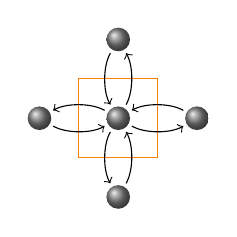
\begin{tikzpicture}[baseline, shorten >=2mm, shorten <=2mm]
    \foreach \point in {(0, 0), (-1, 0), (1, 0), (0, -1), (0, 1)} {
        \shade [ball color=gray] \point circle (1.5mm);
        }
    \draw [orange] (-0.5, -0.5) rectangle (0.5, 0.5);
    \foreach \point in {(-1, 0), (1, 0), (0, -1), (0, 1)} {
        \draw [<-] \point to [bend left]  (0, 0);
        \draw [->] \point to [bend right] (0, 0);
        }
\end{tikzpicture}

        \caption{unit cell}
        \label{square-lattice unit cell}
    \end{subfigure}%
    \begin{subfigure}[b]{4.666cm}
        \input{results/square_lattice/square_lattice_dispersion.sl}
        \caption{dispersion}
        \label{square-lattice dispersion}
    \end{subfigure}%
    \begin{subfigure}[b]{4.666cm}
        \input{results/square_lattice/square_lattice_dos.sl}
        \caption{density of states}
        \label{square-lattice dos}
    \end{subfigure}
    \caption{Properties of the tight-binding square lattice}
\end{figure}
%
In order to perform calculations beyond the approximation of a constant density
of states, some kind of model or experimental data which provides the necessary
electronic structure is required. Throughout the present work, a tight-binding
model of a square lattice will be applied for thus purpose. The unit cell with a
single basis atom is depicted in Fig.~\ref{square-lattice unit cell}, where
arrows represent the allowed electronic transitions. The defining
\name{Hamilton} operator in first quantization reads
%
\begin{equation*}
    \op H = -t \sum_{\vec R}
         [ \ket{\vec R + \vec t_1}
         + \ket{\vec R - \vec t_1}
         + \ket{\vec R + \vec t_2}
         + \ket{\vec R - \vec t_2} ]
    \bra{\vec R},
\end{equation*}
%
where the sum goes over all lattice sites $\vec R = n_1 \vec t_1 + n_2 \vec t_2$
with $n_1, n_2 \in \mathds Z$ at which the \name{Wannier} states $\ket{\vec R}$
are localized. $t$ is the nearest-neighbor coupling parameter, $\vec t_1 = (a \
0)$ and $\vec t_2 = (0 \ a)$ are the translation vectors of length $a$, the
lattice constant.

An expansion into \textsc{Bloch} states $\ket{\vec k}$ with $\vec k = (k_x \
k_y)$ via the \name{Fourier} transform
%
\begin{equation*}
    \ket{\vec R} = \int \D \vec k \, \E^{-\I \vec k \vec R} \ket{\vec k},
\end{equation*}
%
where the integration is e.g. over the first \name{Brillouin} zone, leads to the
dispersion relation
%
\begin{equation*}
    \epsilon(\vec k) = -2 t [\cos(k_x a) + \cos(k_y a)]
\end{equation*}
%
a contour plot of which is given in Fig.~\ref{square-lattice dispersion}.

Finally, the corresponding density of states per spin and unit cell, shown in
Fig.~\ref{square-lattice dos}, reads
%
\begin{equation*}
    n(\epsilon) = \frac{K \big(1 - (\tfrac \epsilon {4 t})^2 \big)}{2 \pi^2 t}
    \quad \text{where} \quad
    K(x) = \int \from 0 \till{\frac \pi 2} \D \varphi \,
    \big[ 1 - x \sin^2(\varphi) \big]^{-\frac 1 2}
\end{equation*}
%
is the complete elliptic integral of the first kind \cite[Eq.~4.146 and
4.147]{Czycholl08}. It features a \textsc{van Hove} singularity at the
\textsc{Fermi} level $\epsilon = 0$ at half-filling, at which is diverges
logarithmically \cite[Eq.~7]{Szczesniak06}. Since the density of states at the
chemical potential of the non-interacting system enters in the definition of the
coupling strengths in Eq.~\ref{coupling strengths}, which have to be finite,
well-defined quantities, a reduced particle number, namely quarter-filling, is
chosen in the following.

\section{Self-energy on real and imaginary axis}

\begin{figure}
    \small
    \input{results/self-energy/Delta(iomega).sl}
    \input{results/self-energy/Delta(omega).sl}
    \input{results/self-energy/chi(iomega).sl}
    \input{results/self-energy/chi(omega).sl}
    \input{results/self-energy/Z(iomega).sl}
    \input{results/self-energy/Z(omega).sl}
    \caption[Self-energy on both complex axes at different temperatures]{
        Imaginary- and real-axis self-energy components at different
        temperatures for a square-lattice density of states with an electronic
        bandwidth of $2 \, \unit{eV}$ at quarter-filling, a phonon frequency
        $\omega \sub E = 20 \, \unit{meV}$, an electron-phonon coupling strength
        $\lambda = 1$, a \name{Coulomb} pseudo-potential $\mu^* = 0.1$ and a
        cutoff frequency $\omega_N = 100 \, \omega \sub E$. Note that the
        displayed frequency ranges do not correspond to the cutoff.}
    \label{imaginary- and real-axis self-energy components}
\end{figure}
%
In Fig.~\ref{imaginary- and real-axis self-energy components} numerical
solutions of the local \name{Eliashberg} equations stated in Eqs.~\ref{local
Eliashberg equations} are shown together with the their \name{Padé} approximants
as presented in Section~\ref{Pade approximants}, analytically continued to the
real axis, for different temperatures. For all parameters sets used in this
work, the qualitative appearance of the resulting curves is the same:

On the imaginary-axis not only the renormalization $Z(\I \omega_n)$, in
accordance with Fig.~\ref{validation Pade}, but also the energy gap $\Delta(\I
\omega_n)$ and shift $\chi(\I \omega_n)$ are bell-shaped and centered at the
origin. The first-mentioned are always concave functions whereas the sign of
the latter may change, resulting in a convex curve as in the example.

Asymptotically, the energy gap approaches the negative or vanishing constant
\name{Coulomb} contribution given in Eq.~\ref{constant Coulomb contribution},
the renormalization goes to unity and the energy shift vanishes, but much more
slowly than the former two.

The maybe most characteristic property of the energy gap is its temperature
dependence, further discussed in the subsequent section, through which it is
qualified as an order parameter for the superconducting state. With rising
temperature it decreases with increasing speed towards zero, which is reached,
by definition, at the critical temperature. In principal, this process affects
the magnitude rather than the shape of the curve, resulting in a common zero of
the displayed family of curves or, more precisely, of their analytic
continuations, since naturally only discrete values over the imaginary axis are
taken which in general do not include this very point. Over the same temperature
range, the other two quantities barely change.

On the real axis the shapes turn out to be more complicated. The renormalization
$Z(\omega)$ basically resembles the analytic one, shown in Fig.~\ref{validation
Pade}, the properties of which have already been discussed. One of them, namely
the vanishing imaginary part at frequencies below the renormalized phonon
frequency, are recognized in the energy gap $\Delta(\omega)$ and shift
$\chi(\omega)$ as well. The former even features the aforementioned peaks, in
the vincinity of which the exact behavior of the \name{Padé} approximants is
untrustworthy for being very sensitive to parameter changes. Beyond the peak,
the real and imaginary parts of the energy gap describe arches of opposite
orientation. The asymptotes of all quantities are the same as on the
imaginary-axis, although in the case of the energy shift this does not become
apparent from the depicted detail.

\subsection{Temperature dependence of the order parameter}

\begin{figure}
    \small
    \centering
    \input{results/order_parameter/order_parameter.sl}
    \caption[Temperature dependence of the order parameter]{
        Order parameters. The temperature dependence of leading \name{Matsubara}
        and measurable gap is shown for the same parameter set as in
        Fig.~\ref{imaginary- and real-axis self-energy components}, except for a
        lower cutoff frequency $\omega_N = 15 \, \omega \sub E$. The phase
        transition in characterized by a diverging number of iterations needed
        to reach self-consistency.}
    \label{order parameter}
\end{figure}
%
Leaving the invariant shape of the energy gap on the imaginary frequency axis
out of account, the temperature dependence of its magnitude, represented by its
value at the first \name{Matsubara} frequency, is shown in Fig.~\ref{order
parameter}. It is supplemented by the corresponding curve for the energy gap
which is actually measurable in experiments and defined by the following
fixed-point equation \cite[Eq.~3a]{VidbergSerene77}:
%
\begin{equation*}
    \Delta_0 = \Re[\Delta(\Delta_0)].
\end{equation*}
%
Both curves turn out to be very similar: Starting at absolute zero, they remain
nearly constant at first and subsequently become ever steeper approaching the
critical temperature at which they vanish. They resemble the well-known BCS
result for which changes exponentially and like a square root near $T = 0$ and
$T \sub c$, respectively \cite[Eq.~11.60]{Czycholl08}.

Fig.~\ref{order parameter} also shows how the number of iterations needed to
obtain a self-consistent solution of the \name{Eliashberg} equations increases
drastically at the critical temperature. This is due to the magnitude of the
energy gap converging much slower than its shape \cite[185]{VidbergSerene77}.
Enforcing the normal-state property $\Delta = 0$ yields a similar convergence
rates at $T \sub c$ and any other temperature.

\section{Convergence tests}

\subsection{Cutoff-induced errors of the self-energy}

\begin{figure}
    \small
    \begin{minipage}{4.666cm}
        \input{results/cutoff/Delta_N(iomega).sl}
    \end{minipage}%
    \begin{minipage}{4.666cm}
        \input{results/cutoff/chi_N(iomega).sl}
    \end{minipage}%
    \begin{minipage}{4.666cm}
        \input{results/cutoff/Z_N(iomega).sl}
    \end{minipage}%
    \caption[Cutoff dependence of the self-energy]{
        Dependence of the shape of the self-energy components on the
        \name{Matsubara} cutoff frequency. Except for the latter, the settings
        are as for the results displayed in Figs.~\ref{imaginary- and real-axis
        self-energy components} and \ref{order parameter}.}
\end{figure}

\begin{itemize}
    \item numeric: $Z(\I \omega_n)$, $\Delta(\I \omega_n)$, $\chi(\I \omega_n)$
    \item analytic: $Z(\I \omega_n)$
\end{itemize}

\subsection{Convergence of critical temperature}

\begin{figure}
    \small
    \begin{subfigure}{7cm}
        \input{results/convergence/cutoff_frequency.sl}
        \caption{square lattice at quarter-filling}
    \end{subfigure}%
    \begin{subfigure}{7cm}
        \input{results/convergence/cutoff_frequency_cdos.sl}
        \caption{constant density of states}
    \end{subfigure}
    \caption[Convergence with cutoff frequency]{
        Convergence with cutoff for a phonon frequency $\omega \sub E = 20 \,
        \unit{meV}$, an electron-phonon coupling strength $\lambda = 1$ and a
        \name{Coulomb} pseudo-potential $\mu^* = 0.1$. In each panel, the latter
        is rescaled differently.}
\end{figure}

\begin{figure}
    \small
    \centering
    \input{results/convergence/integration_points.sl}
    \caption[Convergence with number of integration points]{
        Convergence with the number of integration points for two different
        phonon frequencies. Constants are defined as in Fig.~\ref{order
        parameter}.}
\end{figure}

\section{\name{McMillan}'s equation for \name{Einstein} spectra}

\begin{table}
    \centering
    \input{results/mcmillan/mcmillan.dat}
    \caption{
        $T \sub c \pm 0.001\,\unit K$ for different $\lambda$ and $\mu^*$ with
        $\omega \sub E = 20 \, \unit{meV}$.}
\end{table}

\begin{figure}
    \small
    \begin{subfigure}{7cm}
        \input{results/mcmillan/mcmillan_1st.sl}
        \caption{$\mu^* = 0$}
    \end{subfigure}%
    \begin{subfigure}{7cm}
        \input{results/mcmillan/mcmillan_2nd.sl}
        \caption{$\mu^* > 0$}
    \end{subfigure}
    \caption[\name{McMillan}'s fits]{
        Combined representation of \name{McMillan}'s original data and lines of
        best fit together with their newly calculated counterparts for an
        \name{Einstein} phonon spectrum.}
\end{figure}

\section{Critical-temperature benchmarks}

\begin{figure}
    \small
    \input{results/benchmark/tc_lamda.sl}
    \input{results/benchmark/tc_lamda_2.sl}
    \input{results/benchmark/tc_omegaE.sl}
    \input{results/benchmark/tc_muStar.sl}
    \caption[Critical-temperature benchmarks]{
        Comparison of the critical temperatures according to \name{McMillan}'s
        formula in its original form and with its constants adjusted to an
        \name{Einstein} phonon spectrum as well as the local \name{Eliashberg}
        equations, either within the approximation of a constant density of
        states or for a square lattice with an electronic bandwidth of $2 \,
        \unit{eV}$ at quarter-filling. As constants, an \name{Einstein}
        frequency $\omega \sub E = 20 \, \unit{meV}$, an electron-phonon
        coupling $\lambda = 1$ and a \name{Coulomb} pseudo-potential $\mu^* =
        0.15$ are chosen. The \name{Matsubara} sum is cut off at $\omega_N = 15
        \, \omega \sub E$. 2001 points were used for the numerical solution of
        the energy integral.}
\end{figure}

\section{Dependence on density of states and occupancy}

\begin{figure}
    \small
    \centering
    \input{results/energy/energy_dos.sl}
    \input{results/energy/energy_shift.sl}
    \input{results/energy/energy_tc.sl}
    \caption[Energy dependence of the critical state]{
        Energy dependence. It is shown how the critical temperature, the
        self-consistent chemical potential and the leading energy shift change
        with the chemical potential of the non-interacting system. Again, the
        parameters are the same as in Fig.~\ref{order parameter}.}
\end{figure}

\begin{itemize}
    \item energy shift and chemical potential as function of the initial value
          of the latter
    \item non-well-defined coupling constants because of:
    %
    \begin{itemize}
        \item steep slope of the density of states
        \item non-representative density of states at \name{Fermi} level
    \end{itemize}
\end{itemize}
